The following chapter will describe the methods, implementation details and strategies used to create GPU support for KAGE.

The KAGE genotyping pipeline consists of several steps. 
An abstract overview of the KAGE pipeline can be represented by the following two steps:
\begin{compactenum}
  \item
    Read the input fasta file, extract and encode all valid \textit{k}mers and count the observed \textit{k}mer frequencies of the predetermined set.
  \item
    Determine the genotypes based on the observed \textit{k}mer frequencies.
\end{compactenum}

\begin{figure}[!ht]\label{figure:KAGE-pipeline}
\begin{center}
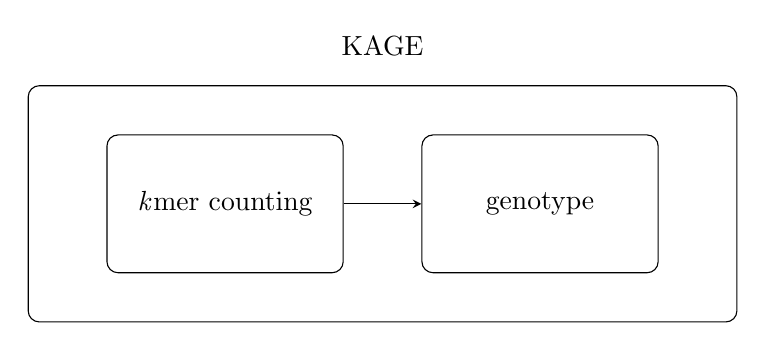
\begin{tikzpicture}
  % draw kmer counting box
  \node at(-2,0)[rectangle,draw,rounded corners,minimum height=1.75cm,minimum width=3cm](kmercounting){\textit{k}mer counting};
  % draw genotype box
  \node at(2,0)[rectangle,draw,rounded corners,minimum height=1.75cm,minimum width=3cm](genotype){genotype};
  % draw "KAGE" text
  \node at(0,2){KAGE};
  % draw KAGE box
  \node at(0,0)[rectangle,draw,rounded corners,minimum width=9cm,minimum height=3cm](kage){};
  % draw arrow from kmer counting to genotype
  \draw [-stealth](kmercounting) -- (genotype);
\end{tikzpicture}
\caption{...}
\end{center}
\end{figure}
